\documentclass[
  aps,prl,reprint,superscriptaddress,
  amsmath,amssymb,floatfix,nofootinbib
]{revtex4-2}
\usepackage{graphicx}
\usepackage{bm}
\usepackage[colorlinks=true,linkcolor=blue,citecolor=blue,urlcolor=blue]{hyperref}
\usepackage{fontawesome5}

\newcommand{\meV}{\,\mathrm{meV}}
\newcommand{\gagg}{g_{a\gamma\gamma}}
\newcommand{\Qm}{Q_{\rm m}}
\newcommand{\Qr}{Q_{\rm r}}
\newcommand{\dd}{\mathrm d}

\renewcommand{\topfraction}{0.98}
\renewcommand{\textfraction}{0.02}
\renewcommand{\floatpagefraction}{0.9}
\begin{document}

\title{Layered Wire-Grid Haloscope for Millielectronvolt Axions and Dark Photons}

\author{Andrea Caputo}
\affiliation{Department of Theoretical Physics, CERN, Esplanade des Particules 1, P.O. Box 1211, Geneva 23, Switzerland}
\affiliation{School of Natural Sciences, Institute for Advanced Study, Princeton, NJ 08540, USA}
\affiliation{Dipartimento di Fisica, ``Sapienza'' Universit\`a di Roma \& Sezione INFN Roma1, Piazzale Aldo Moro 5, 00185, Roma, Italy}

\date{\today}
\begin{abstract}
We propose MADGRID (\textbf{M}illielectronvolt \textbf{A}xions and \textbf{D}ark photons with layered \textbf{GRID}s), a few wire grids in front of a mirror, tuned by their spacing, forming an epsilon-near-zero slab that radiates through its face into external optics. Unlike wire-plasma haloscopes, the signal need not cross the lossy medium to reach an antenna, and metal grids replace the disks of dielectric haloscopes. A 1\,m$^2$ array in 10\,T could probe axion-photon couplings below the CAST bound up to 1.9\,meV with kinetic-inductance detectors, and KSVZ couplings over 0.8--3.9\,meV with future photon counters. Without a magnet, it could probe dark-photon mixings down to $3\times10^{-16}$. The codes used in this work are available on GitHub~\href{https://github.com/andrea0292/Wiregrid_Haloscope}{\faGithub}.
\end{abstract}


\maketitle

\begin{figure}[t]
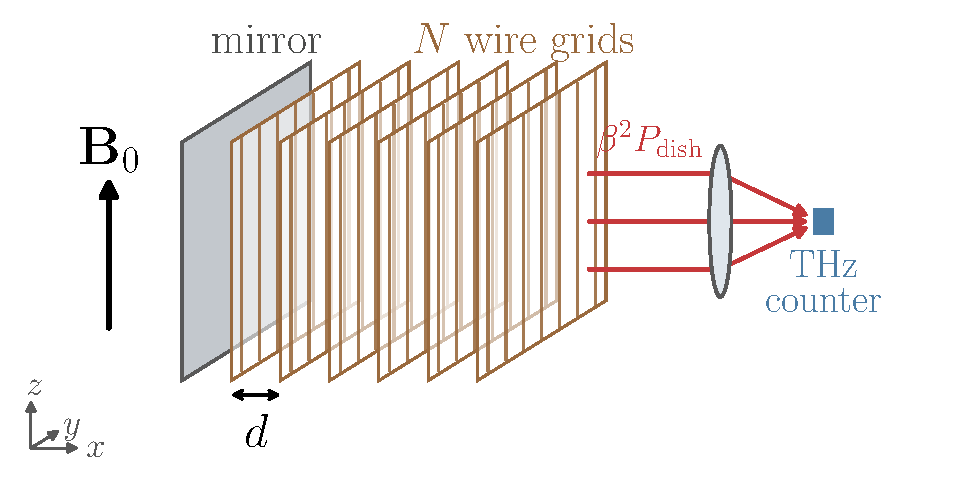
\includegraphics[width=0.9\columnwidth]{fig1.pdf}
\caption{A mirror and $N$ grids of wires parallel to $\mathbf B_0$, at spacing $d$, form an epsilon-near-zero (ENZ) slab. On resonance the slab radiates the power $|\beta|^2P_{\rm dish}$ through its face, where $P_{\rm dish}$ is the power emitted by a bare mirror of the same area and $|\beta|^2$ is the power boost. External optics focus it onto a THz detector.}
\label{fig:concept}
\end{figure}


\textit{Introduction.}---The QCD axion is a very well motivated new particle, introduced to explain why the strong interactions conserve CP~\cite{Peccei:1977hh,Weinberg:1977ma,Wilczek:1977pj}, and subsequently recognized as one of the most appealing dark matter (DM) candidates~\cite{Preskill:1982cy,Abbott:1982af,Dine:1982ah, OHare:2024nmr, Caputo:2024oqc, Safdi:2022xkm}. It couples to photons through the interaction $\mathcal L\supset\gagg a\,\mathbf E\cdot\mathbf B$, with a coupling proportional to its mass, $|\gagg|\simeq2.04\times10^{-13}|C_{a\gamma}|(m_a/{\rm meV})\,{\rm GeV}^{-1}$, where $|C_{a\gamma}|=1.92$ in the KSVZ model~\cite{Kim:1979if,Shifman:1979if} and 0.75 in the DFSZ-I model~\cite{Dine:1981rt,Zhitnitsky:1980tq,DiLuzio:2020wdo}. The mass itself is not predicted by the model. However, if the Peccei--Quinn symmetry is broken after inflation, simulations of the axion-string network point to $m_a\sim0.04$--$0.45\meV$~\cite{Buschmann:2021sdq,Saikawa:2024bta,Benabou:2024msj} or larger values~\cite{Gorghetto:2020qws}, so masses around a meV are motivated. They are also largely unexplored by axion haloscopes.%; a search near 0.11\,meV illustrates the progress toward this range~\cite{Quiskamp:2023ehr}, and a cavity search read out by kinetic-inductance detectors is being prepared near 0.4\,meV~\cite{Aja:2022csb}. %Strong constraints on the photon coupling come from the CAST helioscope~\cite{CAST:2024eil}, from stars in globular clusters~\cite{Dolan:2022kul} and, at the lowest masses, from solar axions observed by NuSTAR~\cite{Ruz:2024gkl}; at 1\,meV the CAST and globular-cluster bounds lie 120--380 times above the QCD prediction.

The difficulty at these masses is mostly geometric. In a magnetic field $\mathbf B_0$, axion DM drives a weak electric field $\mathbf E_a=-\gagg a\mathbf B_0$ that oscillates at $\nu=m_a/(2\pi)$, i.e., 242\,GHz per meV, with amplitude $E_0=\gagg a_0B_0$. Because DM is nonrelativistic, this field is nearly uniform across the depth of any device considered here. A conducting mirror placed in it must cancel the tangential field at its surface, and it does so by emitting a plane wave perpendicular to its face, with power per unit area~\cite{Horns:2012jf}
\begin{equation}
\frac{P_{\rm dish}}{A}=\frac{7.33\times10^{-26}\,{\rm W}}{\rm m^2}\left(\frac{\gagg\,{\rm GeV}}{10^{-12}}\,\frac{B_0}{10\,{\rm T}}\,\frac{\rm meV}{m_a}\right)^{\!2}\!\rho_{0.4},
\label{eq:dish}
\end{equation}
where $\rho_{0.4}=\rho_a/(0.4\,{\rm GeV\,cm^{-3}})$. A resonant cavity would amplify this signal, but at 1\,meV the wavelength is $\lambda=1.24\,$mm, and a cavity resonant at this wavelength collects the signal from a tiny volume. Searches at high mass therefore keep a large converting area and enhance its emission in other ways. Dish antennas focus the emission of a bare mirror~\cite{Horns:2012jf,BREAD:2021tpx}, dielectric haloscopes place a stack of dielectric disks in front of the mirror, which shapes the photon mode so that it overlaps coherently with the axion field~\cite{Caldwell:2016dcw,Millar:2016cjp,MADMAX:2019pub}, while epsilon-near-zero (ENZ) media use a resonance of the material, where its permittivity is nearly zero~\cite{Schutte-Engel:2021bqm,Marsh:2022fmo,Mehrani:2025ryc}.

Plasma haloscopes realize the last idea with an engineered material~\cite{Lawson:2019brd,ALPHA:2022rxj}. For an electric field along the wires, a lattice of thin parallel wires responds like a plasma whose plasma frequency is set by the wire spacing, so it can be matched to the axion mass independently of the size of the device, and the axion excites the plasma oscillation coherently over the whole volume. At meV masses the problem is to get the signal out. In existing designs an antenna inside or at the edge of the medium collects the signal, which therefore has to propagate through the wire medium to reach it. At THz frequencies the wires are lossy, and the Drude response at the plasma frequency gives a field-amplitude $1/e$ attenuation length $\ell_{\rm amp}\simeq\lambda\sqrt{2Q_u}/2\pi$, consistent with the decay length $\sim\sqrt{Q}\,\lambda$ estimated in Ref.~\cite{ALPHA:2022rxj}, where $Q_u$ is the unloaded (that is to say, including only internal losses, here the ohmic dissipation in the wires) quality factor of the medium~\cite{ALPHA:2022rxj}. For a square copper-wire lattice with our choice $r/a=0.03$, using the lattice expressions of Ref.~\cite{ALPHA:2022rxj} and the surface resistance adopted below, $Q_u\simeq510\,(m_a/{\rm meV})^{-2/3}$ (about 14\% above the material quality factor $\Qm$ of Eq.~\eqref{eq:plasma} at $d=a$, because the square-lattice expression includes a correction to the inductance per wire), so that $\ell_{\rm amp}\simeq6.3\,{\rm mm}\,(m_a/{\rm meV})^{-4/3}$, i.e., 6.3\,mm at 1\,meV and 0.4\,mm at 8\,meV. A localized pickup therefore samples only a limited region of a large plasma; distributed readout requires additional collection and transmission structures.

In this Letter we let the plasma radiate. We stack a few free-standing wire grids, with the wires parallel to $\mathbf B_0$, about a quarter wavelength apart in front of a mirror (Fig.~\ref{fig:concept}). Near its resonance the stack acts as a thin ENZ slab, the axion-induced field is enhanced inside it, and the signal leaves through the whole face of the stack into the vacuum in front of it, where ordinary mirrors and lenses collect it without lateral transport to an internal pickup. The same radiative principle underlies SQWARE~\cite{Mehrani:2025ryc}, where the ENZ medium is a GaAs/AlGaAs quantum-well stack of 9--25\,cm$^2$ face tuned in a 36--50\,T field. Wire grids instead reach a large conversion area at 10\,T by repeating tiles of a conventional conductor, tuned mechanically. The same converter can also search for dark photons without a magnet. 

Geometrically, our converter is closest to a dielectric haloscope such as MADMAX~\cite{Caldwell:2016dcw,MADMAX:2019pub}, an open, mirror-backed stack of mechanically positioned layers that radiates through its face into external optics, and replaces its dielectric disks by wire grids. Like any haloscope, both shape the photon mode so that it overlaps with the spatially uniform axion field~\cite{Ioannisian:2017srr,Egge:2023cos}, but in different ways. Dielectric disks have a refractive index above unity, and in resonant configurations disks about half a wavelength apart give a field of nearly the same sign throughout, with shallow reversals in and around the disks~\cite{Millar:2016cjp}. The grids, about a quarter wavelength apart, instead act as inductive sheets, like thin layers of negative permittivity, so that just above the band edge of the lattice the stack has a refractive index close to zero and a long internal wavelength, and its field keeps the same sign throughout. End Matter B discusses the relation to earlier proposals and the role of the readout architecture.


\textit{Mechanism.}---A grid of thin wires of radius $r$ and pitch $a$ is, for fields along the wires, a sheet of impedance $Z_g=R_g-i\omega L_g$, with $L_g=(a/2\pi)\ell$, $\ell=\ln(a/2\pi r)$~\cite{Marcuvitz:1951,Belov:2003}, and $R_g=r_sa/(2\pi r)$ from the wire resistance. Here impedances are normalized to the vacuum impedance $Z_{\rm vac}\simeq376.73\,\Omega$, and $r_s=R_s/Z_{\rm vac}$ is the dimensionless surface resistance corresponding to the physical value $R_s$ quoted below. A stack of grids at spacing $d$ therefore behaves as a Drude medium~\cite{Pendry:1996} (End Matter A), with
\begin{equation}
\varepsilon=1-\frac{\omega_p^2}{\omega(\omega+i\Gamma)},\qquad \omega_p^2=\frac{2\pi}{ad\,\ell},\qquad \Gamma=\frac{r_s}{r\ell},
\label{eq:plasma}
\end{equation}
and a material quality factor $\Qm=\omega_p/\Gamma$,
which coincides with the unloaded quality factor in the
bulk limit when wire resistance dominates the losses. Below $\omega_p$ the medium reflects like a metal, above it transmits like a dielectric, and near $\omega_p$ its permittivity is close to zero. The plasma frequency depends only on the lattice, through $ad$ and $\ell$, and not on the size of the stack, so changing the spacing $d$ tunes it. The losses enter through $\Gamma$, which is small for thick wires of a good conductor. In cold, pure copper the electron mean free path far exceeds the classical skin depth, so we use the extreme anomalous skin-effect limit, in which the surface resistance is independent of the dc resistivity and grows as $\nu^{2/3}$~\cite{ReuterSondheimer:1948}. We extrapolate the copper benchmark $R_s=2.9\,{\rm m}\Omega$, calculated at 3.9\,GHz, 4.2\,K and 6\,T~\cite{Posen:2022tbs,Calatroni:2020ase}, with this law and multiply it by 1.8 as an allowance for additional roughness and magnetoresistance losses at 10\,T, giving $R_s=83.6\,{\rm m}\Omega\,(\nu/250\,{\rm GHz})^{2/3}$. At 10\,T the cyclotron frequency of the conduction electrons, about 0.2--0.3\,THz, lies within the search range and $\mathbf B_0$ is parallel to the wire surfaces, so cyclotron effects may modify the surface impedance. The doubled-$R_s$ bands in Figs.~\ref{fig:reach} and~\ref{fig:dp} indicate the sensitivity of the forecasts to this uncertainty, which in-field THz measurements will have to settle.

Why does such a medium enhance the signal? Inside a homogeneous medium of permittivity $\varepsilon$, the
spatially uniform axion-driven field is $-E_0/\varepsilon$ rather than its vacuum value $-E_0$ (End Matter A). Near $\varepsilon=0$, this response is enhanced, but the signal must escape the medium to be detected. We characterize the emitted radiation by the amplitude boost factor $\beta$, defined as the outgoing electric-field amplitude divided by $E_0$, the amplitude emitted by a bare mirror. The corresponding power enhancement is $|\beta|^2$. For a slab of thickness $L$ backed by a mirror, the lossless limit $\varepsilon=\operatorname{Re}\varepsilon
\equiv u$, with $0<u\ll1$ corresponding to a frequency
slightly above the plasma frequency, admits a resonance when the slab spans half an internal wavelength, $L=\lambda/(2\sqrt{u})$, where $\lambda$ is the vacuum wavelength. At this resonance, $\beta=-2/u$ and the enhanced response inside the slab produces an enhanced outgoing wave. Equivalently, by reciprocity $\beta$ is the overlap of the uniform axion source with the field that a wave sent in from the detector sets up in the stack (SM~\cite{SM}). Including the leading effect of absorption, $\varepsilon\simeq u+i/\Qm$, we find the resonant power boost\footnote{This result agrees with the small-permittivity,
weak-loss limit of the mirror-backed slab response of Ref.~\cite{Mehrani:2025ryc}, after accounting
for the polarization projection used there.}
\begin{equation}
|\beta|^2\simeq
\frac{4}{[u+\pi/(2\Qm\sqrt{u})]^2}.
\label{eq:betamax}
\end{equation}
The two terms in the denominator of Eq.~\eqref{eq:betamax} are proportional, with the same factor $\pi/(2\omega\sqrt u)$, to the two rates at which the stored energy decays. In particular, $u$ corresponds to the radiative rate $\gamma_{\rm rad}$, at which energy leaves through the slab face as the signal, and $\pi/(2\Qm\sqrt u)$ to the ohmic rate $\gamma_{\rm ohm}\simeq\Gamma$, at which it is absorbed in the wires. The boost is therefore inversely proportional to the total damping, as for a driven oscillator, and the ratio of the two terms is $x\equiv\gamma_{\rm rad}/\gamma_{\rm ohm}=2\Qm u^{3/2}/\pi$ (End Matter A). A thicker slab (smaller $u$) enhances the field more but releases it more slowly, so $x$ decreases and a larger fraction of the stored energy is absorbed in the wires. The peak boost is largest, $|\beta|^2_{\max}\simeq0.61\,\Qm^{4/3}$, at $x=1/2$, i.e., when the radiative rate is half the ohmic one. For a background-dominated search, the thickness should optimize sensitivity across a frequency interval. We therefore choose the number of grids to maximize $\mathcal I=\int|\beta(\nu)|^4\,\dd\nu/\nu$, which accounts for both the signal enhancement and its bandwidth (End Matter A).


The homogeneous-slab description explains the enhancement and the balance between radiation and absorption, but it assumes a small phase advance between successive grids, $kd\ll1$, with $k=\omega=2\pi/\lambda$. In the designs below $kd\simeq1.35$--2.1, so the grids are roughly a quarter of a vacuum wavelength apart and propagation across each gap must be treated explicitly. We therefore obtain the design parameters and boost curves by solving the boundary conditions for $N$ impedance sheets $Z_g$ in front of the mirror, retaining the phase accumulated between grids and their multiple reflections. To test the sheet approximation, we also solve Maxwell's equations for arrays of individual circular copper wires, including their coupling within and between grids, with numerical methods and comparisons described in the Supplemental Material (SM)~\cite{SM}.

\textit{Designs.}---For geometrically similar lattices, increasing the target axion mass requires smaller wire radii and spacings. At fixed $r/a$ and $d/a$, Eq.~\eqref{eq:plasma} gives $a\propto m_a^{-1}$. Together with the assumed copper surface resistance $R_s\propto\nu^{2/3}$, this implies $\Qm\propto m_a^{-2/3}$. The optimal slab thickness scales as $L_{\rm opt}\propto\lambda\Qm^{1/3}$, so the preferred number of grids, $N=L/d$, decreases slowly with mass, $N_{\rm opt}\propto\Qm^{1/3}$. These relations guide the choice of dimensions, with the final designs obtained from the discrete-grid calculation. To characterize the bandwidth of each design, we also define the response quality factor $\Qr=\nu_{\rm res}/\Delta\nu_{\rm FWHM}$, where $\nu_{\rm res}$ is the resonant frequency and $\Delta\nu_{\rm FWHM}$ is the full width at half maximum of the power response $|\beta(\nu)|^2$. $\Qr$ describes the resonance of the complete stack, including both radiation escaping through its open face and absorption in the wires. A larger $\Qr$ therefore corresponds to a narrower resonance. 

Table~\ref{tab:design} lists five tunable grid stacks, or cartridges, covering successive factor-of-two intervals in axion mass. Each cartridge has a fixed wire geometry and number of grids and is tuned by varying their separation. To select the grid number, we compare designs with $N$ between 3 and 30, keeping the resonance at the center of each mass band. Figure~\ref{fig:tuning}(a) compares the normalized peak boost and scan response as functions of $x$. For $x>1$, radiation is the dominant decay channel, but for $x<1$, most of the energy is absorbed in the wires. %Expressed in terms of this ratio, 
The numerical results for the five cartridges agree well with the slab model.

Within each cartridge, the wire radius $r$, pitch $a$, and number of grids $N$ remain fixed. We tune the resonance by changing the common separation $d$ between successive grids, including the gap between the mirror and the first grid; compressing the stack raises the resonant frequency. The discrete-sheet calculation shows that covering each assigned interval requires reducing $d/a$ from approximately 1.69 to 0.57. Figure~\ref{fig:tuning}(b) shows the peak power boost at each tuning setting, with its maximum and minimum differing by only a factor of 1.3--1.5 within each cartridge in the sheet model. 

Tuning moves all gaps together, keeping the grids flat and parallel and each setting stable during a measurement. A common drift of 0.13--0.43\,$\mu$m lowers the on-resonance power by 10\%, so the gaps must be held or monitored at this level, with the residual drift absorbed in the scan. Cryogenic variable-delay polarization modulators already move a wire grid relative to a mirror with sub-micron capacitive readout~\cite{Chuss:2014piper}, although over a 1\,mm throw rather than the 16\,mm required by our lowest cartridge. Sagging or tilted grids instead shift the local resonance across the aperture and degrade the coherence of the collected signal, and rms errors of $6\,\mu$m in the lowest cartridge and $0.7\,\mu$m in the highest raise the required coupling by 5\% (SM~\cite{SM}). Tungsten-wire grids have been built with rms spacing and flatness errors below $5\,\mu$m over 100\,mm diameters~\cite{Nagler:2015xta}, which meets the first requirement, while the second calls for a sevenfold improvement.



\begin{figure*}[t]
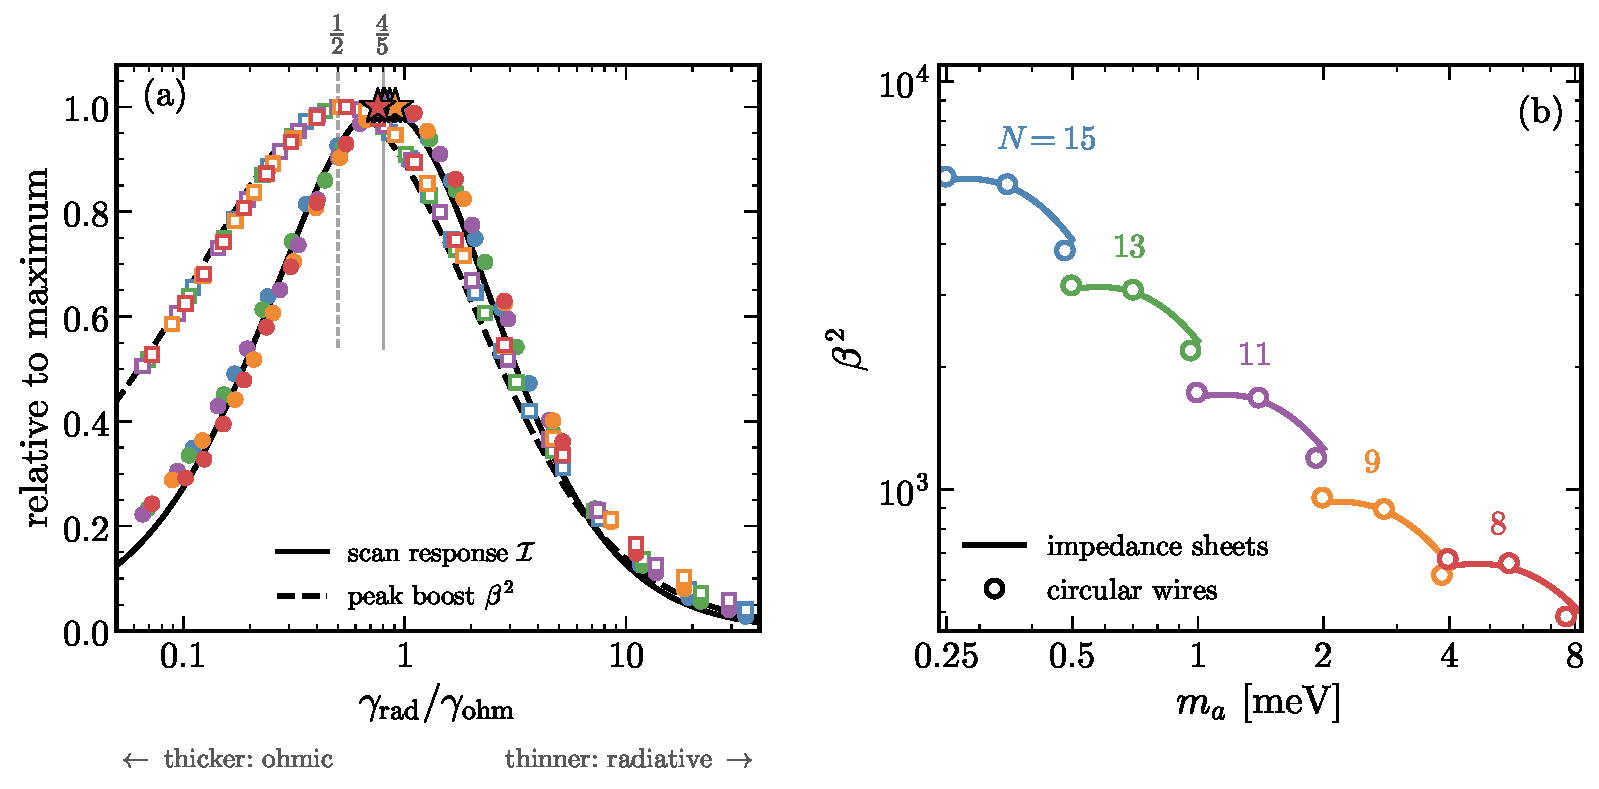
\includegraphics[width=0.92\textwidth]{fig2.pdf}
\caption{Choosing the number of grids and tuning the five cartridges of Table~\ref{tab:design}, one color per cartridge. (a) Grid numbers $N=3$--30, with $d=a$ and lattice dimensions adjusted to keep the resonance at each geometric band center. The horizontal axis is the ratio $x=\gamma_{\rm rad}/\gamma_{\rm ohm}$, extracted from the sheet calculation. Circles show $\mathcal I$ and squares the peak power boost, each normalized to its maximum within that band. Solid and dashed curves are the normalized slab predictions, with maxima at $x=4/5$ and $1/2$, respectively. Stars mark the selected designs. (b) Peak power boost as each cartridge is tuned by varying $d$ at fixed $a$, $r$, and $N$ (labels). Lines give the sheet prediction; open circles show the circular-wire calculation.}
\label{fig:tuning}
\end{figure*}

\begin{table}[t]
\caption{Benchmark cartridges for five successive mass intervals. Each cartridge has a fixed wire pitch $a$, wire diameter $2r$ and grid number $N$, the latter chosen to maximize the scan response $\mathcal I$ among the sampled designs. The thickness $L=Nd$, the material and response quality factors $\Qm$ and $\Qr$, and the peak power boost $|\beta_{\rm pk}|^2$ are evaluated at the geometric center of each interval, where $d=a$, with $R_s$ taken at the resonance frequency. We use $r=0.03a$ except in the 4--8\,meV cartridge, where this scaling would require wires about $3.6\,\mu{\rm m}$ in diameter. There we take instead $2r=5\,\mu{\rm m}$, as in free-standing tungsten grids~\cite{Ade:1979,Mok:1979}, and adjust the pitch to keep the target resonance. All designs assume copper (or copper-coated) wires with the surface resistance adopted in the text.}
\label{tab:design}
\begin{ruledtabular}
\begin{tabular}{lcccccc}
Band [meV] & $N$ & $a$ [$\mu$m] & $2r$ [$\mu$m] & $L$ [mm] & $\Qm$ & $\Qr$\,/\,$|\beta_{\rm pk}|^2$\\
\hline
0.25--0.5 & 15 & 946 & 56.7 & 14.2 & 895 & 585\,/\,5530\\
0.5--1 & 13 & 474 & 28.4 & 6.16 & 564 & 379\,/\,3040\\
1--2 & 11 & 238 & 14.3 & 2.61 & 355 & 239\,/\,1650\\
2--4 & 9 & 120 & 7.17 & 1.08 & 224 & 146\,/\,883\\
4--8 & 8 & 63.7 & 5.00 & 0.510 & 169 & 123\,/\,641
\end{tabular}
\end{ruledtabular}
\end{table}

\textit{Collection.}---The preceding calculation treats the stack as finite in thickness but infinite in its plane. To determine the power reaching a receiver, we instead consider a square tile of side $W$, with the wires along $y$ and the grid normal along $z$, viewed through optics that couple to a single Gaussian spatial mode of waist radius $w\simeq W/2$, at which the field amplitude falls to $1/e$ of its central value. As in three-dimensional studies of dielectric haloscopes~\cite{MADMAX:2021lxf}, the received power is set by how well the emitted field matches this mode in amplitude and phase, rather than by the total radiated power. We compute this overlap with a model that resolves the individual wires across the tile and the finite mirror, treating the field along the wires paraxially. At the tested settings $74$--$78\%$ of the periodic-model power reaches the Gaussian mode, and an independent mode-matching calculation gives a comparable bandwidth-weighted collection factor. We adopt $\eta_{\rm ap}=0.65$, leaving some margin below these values, and describe the sampled geometries and the limitations of both calculations in the SM~\cite{SM}.

Axion motion further reduces the collected signal. A velocity component parallel to the tile face produces a phase gradient in the driving current, which slightly tilts the emitted beam away from the fixed receiver mode. We include this through a factor $\xi$, the halo-averaged collected power relative to the zero-velocity result. To limit this dephasing we use 10\,cm tiles up to 4\,meV and 5\,cm tiles above, giving $\xi\simeq0.76$--$1$ across the search range for the adopted halo model, with the mean wind in the tile plane, the least favorable orientation~\cite{SM}.

\textit{Sensitivity.}---Each tile feeds its own detector, with signal power
\begin{equation}
P_s=\eta_d\eta_{\rm ap}\xi|\beta|^2P_{\rm dish},
\end{equation}
where $P_{\rm dish}$ is the power from a bare mirror of the same area. The efficiency $\eta_d$ is the product of the transmission through the receiving optics and the detector efficiency, after the collection losses already included in $\eta_{\rm ap}$ and $\xi$. We adopt $\eta_d=0.5$ as a requirement on this combined chain. For photon counting this means half of the photons entering the collected spatial mode must produce registered events. Microwave photon counters have reached comparable operational efficiencies~\cite{Balembois:2023bvs,Braggio:2024xed}, an optical efficiency of about 0.9 has been inferred for quantum-capacitance detectors at $1.5\,{\rm THz}$~\cite{Echternach:2017vtf}, and BREAD adopts the same signal efficiency~\cite{BREAD:2021tpx}.

Our reference array has an active area $A=1\,{\rm m^2}$ at $0.1\,{\rm K}$ in a field $B_0=10\,{\rm T}$, a magnet benchmark motivated by BREAD and MADMAX concepts~\cite{BREAD:2021tpx,MADMAX:2019pub}. Because the wires must be parallel to $\mathbf B_0$ while the signal leaves normal to the grids, the array requires a field parallel to the tile faces, as provided by the dipole planned for MADMAX, with the optical channels guided to detectors outside the high-field region. We allocate $T_{\rm oct}=1\,{\rm yr}$ of live observing time to each factor-of-two interval in mass, shared among tuning settings uniformly in logarithmic frequency, so that the five-octave search requires a total of five years. Sensitivities combine all tiles and settings at a local signal-to-noise ratio of 5 (End Matter B).

We consider three readouts. Heterodyne receivers resolve the axion line, of effective width $\Delta\nu_a=10^{-6}\nu$, and we assign them up to $4\,{\rm meV}$ ($0.97\,{\rm THz}$) a noise power spectral density $N_{\rm sys}=10\,\omega$, an approximate single-sideband benchmark motivated by ALMA receivers~\cite{Uzawa:2021,Kerr:2014alma,Baryshev:2015alma}. For kinetic-inductance detectors (KIDs), used as power detectors, we adopt a one-sided, absorbed-power-referred ${\rm NEP}=3\times10^{-19}\,{\rm W/\sqrt{Hz}}$ per channel, motivated by kilo-pixel measurements near $0.85\,{\rm THz}$ and detector development for $1.4$--$2.8\,{\rm THz}$~\cite{Baselmans:2017kid,Bueno:2018kid}. These demonstrations overlap the upper search band, and maintaining the same noise at lower frequencies is a development target, requiring adapted optical coupling and, below the aluminium pair-breaking threshold of about $0.39\,{\rm meV}$, a lower-gap absorber. For photon counters we assume the combined efficiency defined above and a dark-count rate $D_{\rm dark}=1\,{\rm mHz}$ per channel, as reached by quantum-dot counters~\cite{Komiyama:2000,Ikushima:2010}, giving a total background of $0.1\,{\rm s^{-1}}$ for the 100 channels of $10\,{\rm cm}$ tiles and $0.4\,{\rm s^{-1}}$ for the 400 channels of $5\,{\rm cm}$ tiles above $4\,{\rm meV}$. These forecasts assume stationary Poisson backgrounds of known mean, with cold, filtered optics keeping thermal photons below the dark rate. The stack itself absorbs nearly all the power incident in the collected mode and thus also emits thermally into it, an emission that stays below 10\% of the dark rate only if the stack is colder than about 0.4\,K at 1\,meV and 0.1\,K at the bottom of the lowest cartridge.

Figure~\ref{fig:reach} shows that heterodyne receivers reach below the globular-cluster and CAST bounds up to approximately $1.0\,{\rm meV}$, and KIDs up to $1.6$ and $1.9\,{\rm meV}$, respectively. The assumed counters reach the DFSZ-I benchmark over approximately $0.8$--$1.2\,{\rm meV}$ and the KSVZ benchmark over $0.8$--$3.9\,{\rm meV}$, the lower endpoint being set by their assumed frequency coverage. This QCD reach defines a detector-development target whose ingredients have been demonstrated separately. Quantum-capacitance devices have counted $1.5\,{\rm THz}$ photons with high optical efficiency~\cite{Echternach:2017vtf} and have been fabricated in 441-pixel arrays~\cite{Echternach:2021}, while quantum-dot counters, which achieved the first far-infrared single-photon detection~\cite{Komiyama:2000}, have reached $1\,{\rm mHz}$ at $70\,{\rm mK}$ and 1.5--3\,THz, with efficiencies for coupling from vacuum roughly estimated at $0.1$--$1\%$~\cite{Ikushima:2010}. Qubit-based pair-breaking sensors designed for single THz photons offer a further route~\cite{Fink:2023tvb}. Combining efficient detection with millihertz backgrounds across $0.2$--$2\,{\rm THz}$ remains the main advance required. In the background-dominated regime the signal of the whole array competes with the dark counts of all its channels, so the reach of Eq.~\eqref{eq:counter_scaling} scales as $(N_{\rm ch}D_{\rm dark}/\eta_d^2)^{1/4}$, with $N_{\rm ch}=100$ for $10\,{\rm cm}$ tiles. At low masses this requirement could be relaxed by reducing the number of channels, because the axion coherence length $1/(m_a\sigma_v)\simeq0.4\,{\rm m}\,({\rm meV}/m_a)$ exceeds the tile size and neighboring tiles could be combined into a few modes, each read by one counter~\cite{Jeong:2017xqz}.

To give an idea of how things scale, let us consider an array of $10\,{\rm cm}$ tiles at $m_a=1\,{\rm meV}$, one gets (fixed halo density, converter response, collection factors)
\begin{equation}
\begin{aligned}
g_{\min}\simeq{}&
1.30\times10^{-13}\,{\rm GeV^{-1}}
\left(\frac{10\,{\rm T}}{B_0}\right)
\left(\frac{0.5}{\eta_d}\right)^{1/2}
\\
&\times
\left(\frac{D_{\rm dark}}{1\,{\rm mHz}}\right)^{1/4}
\left(\frac{1\,{\rm m^2}}{A}\right)^{1/4}
\left(\frac{1\,{\rm yr}}{T_{\rm oct}}\right)^{1/4}.
\end{aligned}
\label{eq:counter_scaling}
\end{equation}

%We notice that we stop at 8 meV because a further octave would require wires thinner than the 5 $\mu$m free-standing grids already demonstrated, or thick-wire lattices outside the sheet model, together with sub-micrometer flatness.

\begin{figure}[t]
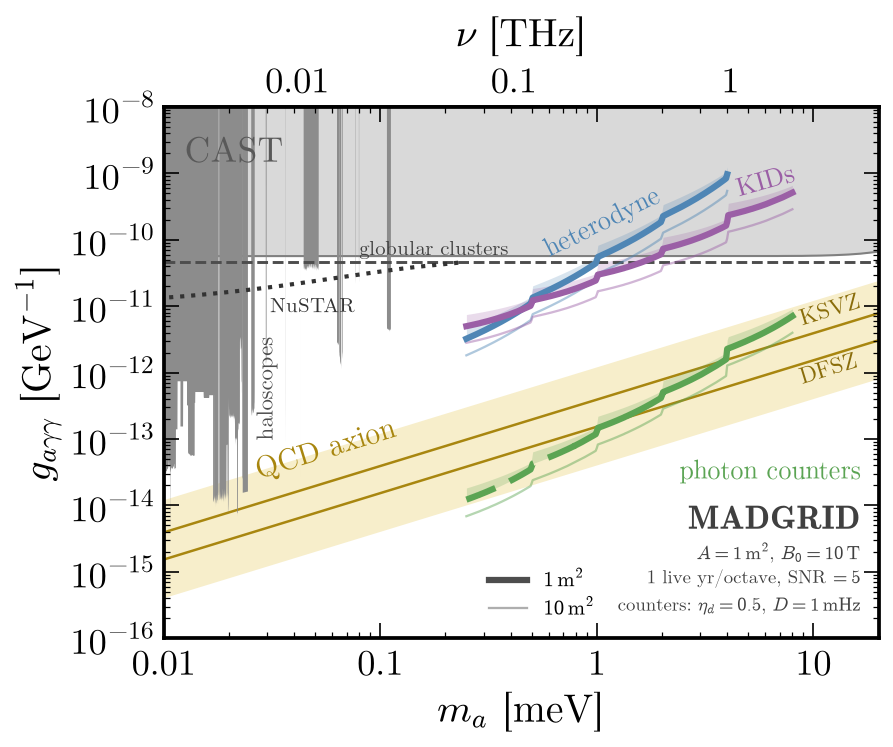
\includegraphics[width=\columnwidth]{fig_axion_1m2_context.png}
\caption{Axion reach (local SNR\,$=5$, one live year per octave) of a 1\,m$^2$ array in 10\,T (thick curves) and of 10\,m$^2$ with the same per-channel detectors and exposure (thin curves). Photon counters assume $\eta_d=0.5$ and $D_{\rm dark}=1\,{\rm mHz}$ per channel, and are dashed below 190\,GHz, where their performance is extrapolated. Colored bands show the effect of doubling $R_s$. Existing bounds are CAST~\cite{CAST:2024eil} (light gray), globular clusters~\cite{Dolan:2022kul} (dashed), NuSTAR observations of the quiet Sun~\cite{Ruz:2024gkl} (dotted), and haloscope searches (dark gray)~\cite{Wuensch:1989sa,ADMX:2018ogs,ADMX:2021mio,CAPP:2020utb,Jeong:2020cwz,Lee:2022mnc,Yang:2023yry,Kim:2023vpo,Bae:2024kmy,Adair:2022rtw,Brubaker:2016ktl,HAYSTAC:2018rwy,HAYSTAC:2020kwv,HAYSTAC:2023cam,HAYSTAC:2024jch,TASEH:2022vvu,Grenet:2021vbb,McAllister:2017lkb,Quiskamp:2022pks,Quiskamp:2023ehr,Quiskamp:2024oet,Alesini:2019ajt,Alesini:2020vny,Alesini:2022lnp,QUAX:2023gop,QUAX:2024fut,CAST:2020rlf,Ahyoune:2024klt,MADMAX:2024sxs,GigaBREAD:2025lzq,AxionLimits}. %The gold band marks QCD axion models, with KSVZ and DFSZ as solid lines.
}
\label{fig:reach}
\end{figure}

\begin{figure}[t]
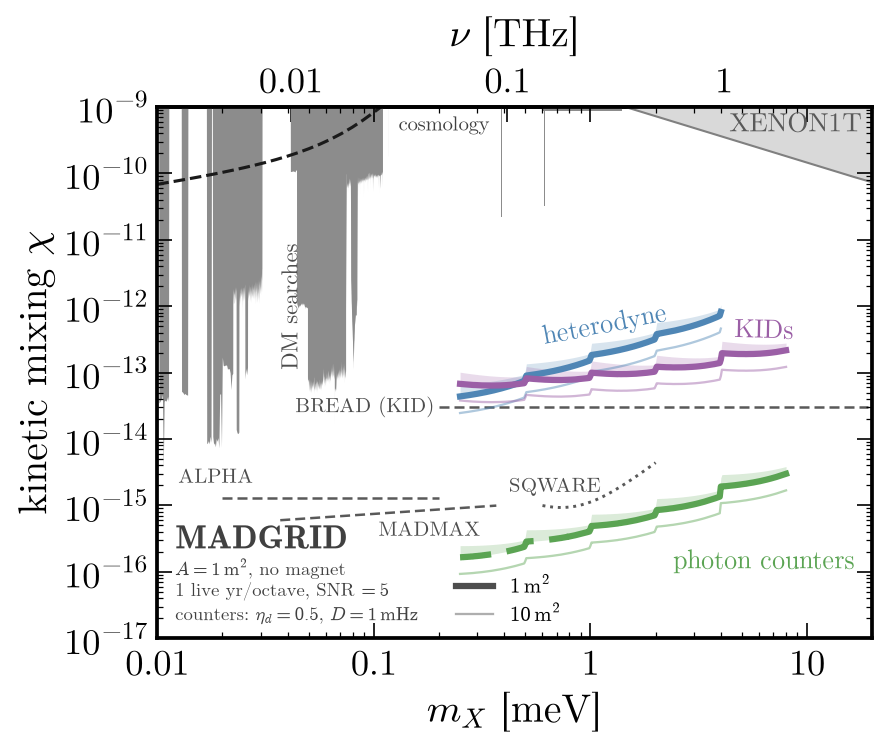
\includegraphics[width=\columnwidth]{fig_dp_1m2_context_proj.png}
\caption{Dark-photon reach of the array without magnet, with curves, bands and dashed extrapolations as in Fig.~\ref{fig:reach}. The light gray region is excluded by solar dark photons in XENON1T~\cite{An:2020bxd}, the dashed black line is the cosmological bound on dark-photon dark matter~\cite{Witte:2020rvb,Caputo:2020bdy}, and dark gray regions are dark-matter searches~\cite{Caputo:2021eaa,Dixit:2020ymh,Brun:2019kak,Ramanathan:2022egk,Schneemann:2023bqc,Bajjali:2023uis,DOSUE-RR:2022ise,DOSUE-RR:2023yml,BREAD:2023xhc,MADMAX:2024jnp,Cervantes:2022yzp,Tomita:2020usq,Knirck:2018ojz,Wei:2025ddp,Fan:2022uwu,Ourahou:2026dandelion,AxionLimits}. Dashed gray lines show projections for a plasma haloscope and MADMAX~\cite{Gelmini:2020kcu} and for BREAD with one KID/TES over 1000 days~\cite{BREAD:2021tpx}, and the dotted line shows the most sensitive SQWARE configuration~\cite{Mehrani:2025ryc}.}
\label{fig:dp}
\end{figure}

\textit{Dark photons.}---The same converter can search for dark-photon DM without an applied magnetic field. A dark photon of mass $m_X$ and dimensionless kinetic mixing $\chi$~\cite{Holdom:1985ag} drives ordinary electric currents through an effective source $\mathbf J_X=\chi m_X^2\mathbf X$. For local density $\rho_X$, its driving-field amplitude along the wires is $\chi\sqrt{2\rho_X}\cos\theta$, where $\theta$ is the angle between the dark-photon polarization and the wires~\cite{Gelmini:2020kcu,Caputo:2021eaa}. Replacing the axion amplitude $\gagg a_0B_0$ by this expression gives %. Assuming the same local density, halo distribution, detector performance and material losses, the axion coupling reach $g_{\min}$ at $m_a=m_X$ therefore maps to
\begin{equation}
\begin{aligned}
\chi_{\min}\simeq{}&
3.38\times10^{-15}
\left(\frac{g_{\min}}{10^{-12}\,{\rm GeV^{-1}}}\right)
\left(\frac{B_{\rm ref}}{10\,{\rm T}}\right)
\\
&\times
\left(\frac{1\,{\rm meV}}{m_X}\right)
\left(\frac{1/3}{\kappa}\right)^{1/2},
\end{aligned}
\label{eq:dpmap}
\end{equation}
where $B_{\rm ref}$ is the field used in the axion forecast and $\kappa=\langle\cos^2\theta\rangle=1/3$ for isotropically randomized polarization. A fixed polarization produces daily modulation as the wires rotate with the Earth, making the sensitivity depend on detector orientation and observing schedule~\cite{Caputo:2021eaa}. We assume randomized polarization and show our results in Figure~\ref{fig:dp}. %gives $\chi_{\min}\simeq9\times10^{-14}$ with KIDs and $(4$--$5)\times10^{-16}$ with the assumed counters near $1\,{\rm meV}$, and the counter reach extends to $3\times10^{-16}$ at the lower end of their assumed frequency coverage. %For comparison, Dandelion constrains $\chi<8.7\times10^{-10}$ over approximately $0.6$--$1.4\,{\rm meV}$~\cite{Ourahou:2026dandelion}, while stronger limits of order $10^{-11}$ have been obtained in narrow intervals near $0.39$ and $0.61\,{\rm meV}$~\cite{Wei:2025ddp,Fan:2022uwu}.

\textit{Conclusions.}---With KIDs at demonstrated noise levels, a 1\,m$^2$ MADGRID array would set the strongest constraints on axions below 2\,meV and on dark photons near 1\,meV. The next steps are a bench demonstration of the tile resonance and its spacing tuning, and a measurement of the in-field THz surface impedance of thin copper wires. THz photon counters with millihertz backgrounds would then bring the QCD axion band within reach.

\textit{Acknowledgments---}
It is a pleasure to thank Valerie Domcke, Anton Ivanov, Bela Majorovits and Georg Raffelt for comments on the draft. This work is supported by an ERC STG grant (``AstroDarkLS'', grant No. 101117510). The author acknowledges hospitality by the Institute for Advanced Study supported by an anonymous donor.


\bibliography{bib}

%\clearpage
\onecolumngrid
\begin{center}{\large\bfseries End Matter}\end{center}
\twocolumngrid
\setcounter{equation}{0}
\renewcommand{\theequation}{A\arabic{equation}}
\renewcommand{\theHequation}{A.\arabic{equation}}

\section*{A. Resonant emission from the wire-grid slab}

The effective-medium description follows by averaging the grid currents over their separation. A sheet carrying surface current $K=E_\parallel/Z_g$ gives a volume current density $J=E_\parallel/(dZ_g)$, where $E_\parallel$ is the electric field along the wires. The stack therefore has an effective conductivity $1/(d  Z_g)$; substituting the resistive and inductive parts of $Z_g$ gives the Drude permittivity in Eq.~\eqref{eq:plasma}. Throughout this discussion, $\varepsilon$ denotes the permittivity along the wires, with the static field $\mathbf B_0$ parallel to them.

For a spatially uniform axion source with time dependence $e^{-i\omega t}$, Amp\`ere's law becomes $-i\omega\varepsilon\mathbf E+\mathbf J_a=0$, where $\mathbf J_a=\gagg\dot a\,\mathbf B_0$. The particular solution is then $\mathbf E=-\gagg a\mathbf B_0/\varepsilon$: the material currents therefore modify the field needed to balance the axion source. This explains the enhancement near $\varepsilon=0$, but a uniform particular solution alone carries no outgoing radiation. The emitted wave must be obtained by imposing the boundary conditions on the driven field and the electromagnetic waves that accompany it.

Let $s$ measure distance normal to a slab occupying $0<s<L$, with a perfect mirror at $s=0$. For the source confined to the slab, the fields along the wires can be written as
\begin{equation}
\begin{aligned}
E_{\rm in}(s)&=\frac{E_0}{\varepsilon}\big[\cos(nks)-1\big]
                +C\sin(nks),\\
E_{\rm out}(s)&=\beta E_0e^{ik(s-L)},
\end{aligned}
\end{equation}
where $n=\sqrt{\varepsilon}$, $k=\omega$, $E_0=\gagg a_0B_0$, and $C$ is a wave amplitude fixed by matching at the face. This form already enforces $E_{\rm in}(0)=0$. Since the permeability is the same on both sides, continuity of the tangential electric and magnetic fields requires $E_{\rm in}(L)=\beta E_0$ and $E'_{\rm in}(L)=ik\beta E_0$, where a prime denotes $\dd/\dd s$. Eliminating $C$ gives
\begin{equation}
\beta=\frac{1-\cos\phi}{\varepsilon\cos\phi-in\sin\phi},
\qquad \phi=nkL.
\label{eq:betaslab}
\end{equation}
Thus $|\beta|^2$ is the emitted power relative to a bare mirror of the same area. For a lossless medium with $\varepsilon=u>0$, the half-wave condition $\phi=\pi$ gives $L=\lambda/(2\sqrt{u})$ and $\beta=-2/u$, where $\lambda=2\pi/k$ is the vacuum wavelength.

Absorption regularizes this enhancement. Slightly above the plasma frequency, write $\varepsilon\simeq u+i/\Qm$, with $\Qm=\omega_p/\Gamma$ and $\Qm^{-1}\ll u\ll1$. At the lossless half-wave condition, the phase becomes $\phi\simeq\pi+i\pi/(2u\Qm)$, so the dominant real part of the denominator in Eq.~\eqref{eq:betaslab} is $-[u+\pi/(2\Qm\sqrt{u})]$. Writing $x=\gamma_{\rm rad}/\gamma_{\rm ohm}$ for the ratio of radiative to ohmic energy-decay rates, the peak amplitude is
\begin{equation}
|\beta_{\rm pk}|\simeq\frac{2}{u+\pi/(2\Qm\sqrt{u})}
=\frac{2}{u}\frac{x}{1+x},
\label{eq:peakescape}
\end{equation}
Squaring this expression gives Eq.~\eqref{eq:betamax} in the main text.

To identify these rates, let $U$ be the stored energy, which decays as $\dot U=-(\gamma_{\rm rad}+\gamma_{\rm ohm})U$ after the drive is removed. For the lossless Drude law, $nk=\sqrt{\omega^2-\omega_p^2}$, so the group velocity $v_g=[\dd(nk)/\dd\omega]^{-1}=\sqrt{u}$ becomes small near the plasma frequency. The power transmission through the face is then $\mathcal T=4\sqrt{u}/(1+\sqrt{u})^2\simeq4\sqrt{u}$. A wave encounters that face once per round trip of duration $2L/v_g$, giving $\gamma_{\rm rad}\simeq\mathcal T v_g/(2L)=2\omega u^{3/2}/\pi$. Together with $\gamma_{\rm ohm}\simeq\Gamma$, this yields
\begin{equation}
x\equiv\frac{\gamma_{\rm rad}}{\gamma_{\rm ohm}}
\simeq\frac{2\Qm u^{3/2}}{\pi},
\qquad \Qr\simeq\frac{\Qm}{1+x}.
\end{equation}
Here $\Qr=\nu_{\rm res}/\Delta\nu_{\rm FWHM}$ describes the full width at half maximum of the power response; the corresponding angular-frequency width is $\gamma_{\rm rad}+\gamma_{\rm ohm}$. Equation~\eqref{eq:peakescape} therefore expresses the lossless enhancement multiplied by the fraction of stored energy that escapes. For the discrete stacks of Table~\ref{tab:design}, whose gaps are not small compared with the wavelength, the ohmic quality factor $Q_{\rm ohm}\equiv\omega/\gamma_{\rm ohm}$ differs from the material parameter $\Qm$. The calculated linewidths give $Q_{\rm ohm}\simeq(1.2$--$1.3)\,\Qm$, with $\Qr\simeq Q_{\rm ohm}/(1+x)$.

A scan also benefits from the bandwidth of the enhancement. In the background-dominated regime the squared signal-to-noise ratio grows as the integration time times the squared signal power, and hence as $|\beta|^4$. Writing $\nu_{\rm res}$ for the tuned resonance frequency, uniform exposure per logarithmic interval means $\dd t=(T_{\rm oct}/\ln2)\,\dd\ln\nu_{\rm res}$, where $T_{\rm oct}$ is the live time per octave. Combining measurements as the resonance passes a fixed axion frequency gives a squared signal-to-noise ratio proportional to $\mathcal I=\int|\beta(\nu)|^4\,\dd\nu/\nu$, provided the detector noise and response shape vary slowly across the resonance. For a narrow Lorentzian,
\begin{equation}
\begin{aligned}
|\beta(\nu)|^2&\simeq\frac{|\beta_{\rm pk}|^2}
 {1+4\Qr^2[(\nu-\nu_{\rm res})/\nu_{\rm res}]^2},\\
\mathcal I&\simeq\frac{\pi|\beta_{\rm pk}|^4}{4\Qr}
\propto\frac{x^{4/3}}{(1+x)^3}.
\end{aligned}
\end{equation}
This expression is maximal at $x=4/5$, and it is this scan optimum, rather than the largest boost alone, that guides the choice of the number of grids. In the forecasts for power detectors we conservatively count only the exposure during which the axion frequency lies within the half-maximum width of the response. For a Lorentzian this retains a fraction $1/2+1/\pi\simeq0.82$ of $\mathcal I$, and it raises the coupling threshold by about 5\%.


For the actual stack, the vacuum gaps are not small compared with the wavelength, so the slab result should be seen only as a scaling guide. In each gap we retain the driven field and both traveling waves, impose continuity of the electric field and the magnetic-field jump due to the sheet current, and apply the mirror and outgoing-wave conditions. Solving this linear system gives $\beta(\nu)$ and $\mathcal I$ without homogenization. Radiative and ohmic linewidths are separated by repeating the calculation with negligible resistance, which gives the radiative quality factor $Q_{\rm rad}$ and $Q_{\rm ohm}^{-1}=\Qr^{-1}-Q_{\rm rad}^{-1}$; the circular-wire checks and the correction for a source extending outside the stack are detailed in~\cite{SM}.


\renewcommand{\theequation}{B\arabic{equation}}
\renewcommand{\theHequation}{B.\arabic{equation}}
\setcounter{equation}{0}
\section*{B. Relation to other proposals}

The tunable wire plasma introduced by Lawson \emph{et al.}~\cite{Lawson:2019brd} underlies the ALPHA program, which also considered operation without an enclosing cavity and readout through multiple antennas~\cite{ALPHA:2022rxj}. Mirror-backed dielectric multilayers are central to MADMAX and DALI~\cite{MADMAX:2019pub,DeMiguel:2020rpn}, and architecturally our converter is closest to them, with wire grids in place of dielectric disks. Both are layered boosters. For lossless dielectric disks the frequency-integrated boost obeys an area law~\cite{Millar:2016cjp}, which does not directly apply to the dispersive and lossy grids. Numerically, integrating over 0.5--1.5 times the design frequency gives $\int|\beta|^2\dd\nu/\nu\simeq2.5$ per sapphire disk ($\varepsilon=9.4$, half-wave configuration) and $\simeq2.6$ per grid for our lossless 1--2\,meV design, reduced to $\simeq1.4$ by the copper losses. 
Per element the two are thus comparable, and they differ mainly in how the mode is sculpted. Dielectric disks about half a wavelength apart have a refractive index above unity, whereas metallic grids about a quarter wavelength apart act as inductive sheets, whose periodic stack has a band edge at its plasma frequency and, just above it, an effective refractive index close to zero. The radiative ENZ mechanism is instead shared with SQWARE~\cite{Mehrani:2025ryc}.

Comparing these approaches requires the signal power delivered to each detector, its noise, and the observing time available at each mass. For independent power-detector measurements with white noise, the squared signal-to-noise ratio is
\begin{equation}
\mathrm{SNR}^2=2\sum_{i,j}
\frac{t_i P_{s,ij}^{\,2}}{{\rm NEP}_j^{\,2}},
\label{eq:comparison_snr}
\end{equation}
where $i$ labels tuning settings, $j$ labels detectors, $t_i$ is the live time at a setting, and $P_{s,ij}$ is the detected signal power. For background-dominated photon counting, the same expression applies upon replacing ${\rm NEP}_j^2$ by $2(2\pi\nu)^2D_j$, where $D_j$ is the background count rate. Dividing a fixed total signal equally among $N_{\rm det}$ independent detectors reduces $\mathrm{SNR}^2$ by $N_{\rm det}$ relative to collecting it onto one detector with the same noise and efficiency, if such collection is physically possible.

For axions at fixed mass and density, the signal power scales as $\gagg^2 B_0^2 A\eta|\beta|^2$, where $\eta=\eta_d\eta_{\rm ap}\xi$ includes collection, transmission and detection efficiency. A scan must also account for the resonance bandwidth, as a larger peak boost need not improve sensitivity if each mass is observed for a correspondingly shorter time. Uniform exposure per logarithmic frequency interval introduces the response integral $\mathcal I$ derived in End Matter A. For identical channels sharing total area $A$, at fixed noise per detector, the coupling reach therefore scales as
\begin{equation}
g_{\min}\propto
\left[
\frac{(\eta B_0^2A)^2\,T_{\rm oct}\mathcal I}
{N_{\rm det}}
\right]^{-1/4}.
\end{equation}
The same statistical argument applies to dark photons, whose signal instead scales with $\chi^2\kappa$, where $\kappa$ is the mean squared polarization projection, without $\gagg^2B_0^2$.

SQWARE uses the same radiative principle with a smaller area, a stronger resonance and a larger field. For its LM and LM-S configurations~\cite{Mehrani:2025ryc}, resonant at 1.53 and 1.07\,meV, we find $\mathcal I\simeq8.5\times10^3$ and $1.0\times10^5$ with $B_0^2A=1.17$ and $6.25\,{\rm T^2m^2}$, against our 100 tiles at $B_0^2A=100\,{\rm T^2m^2}$. Assuming unit collection onto one detector per SQWARE sample, and equal detector noise and time per logarithmic interval, our array reaches couplings 2.4 times smaller than LM, while LM-S reaches couplings 1.9 times smaller than ours. SQWARE, however, requires 2--20\,mm quantum-well structures and 36--50\,T fields, whereas the grids require validation of copper losses, tolerances and collection, and operate without a magnet for dark photons.

For ALPHA and related wire-plasma designs~\cite{Lawson:2019brd,ALPHA:2022rxj}, the geometry and the extraction of the signal both differ. ALPHA fills the bore of a solenoid with a three-dimensional wire metamaterial enclosed in a resonator, tuned by moving the wires of the lattice and read out through an antenna coupled to the resonator, with its first phase targeting 10--20\,GHz~\cite{ALPHA:2026phase1}. At higher frequencies, ohmic attenuation limits the region that one localized antenna can collect efficiently. Additional antennas can recover signal from a larger volume, as discussed by ALPHA~\cite{ALPHA:2022rxj}, but their signals must then be transported to receivers or combined through a collection network. %Our converter is instead a thin, open, mirror-backed stack of a few planar grids, about a quarter wavelength apart and tuned by their spacing, in a field parallel to its face. The plasma mode is confined to a slab a few wavelengths thick, and the signal escapes through the whole face into external optics without propagating over large distances inside the wire medium.

Finally, we compare the dark-photon reach with that of BREAD, which projects $\chi\simeq3\times10^{-14}$ for a $10\,{\rm m^2}$ dish read by one detector with ${\rm NEP}=2\times10^{-19}\,{\rm W/\sqrt{Hz}}$ for 1000\,d~\cite{BREAD:2021tpx}. Our $1\,{\rm m^2}$ KID forecast is about three times weaker near 1\,meV, because it uses a tenth of the area and 100 independent detectors, each adding its own noise, and the resonance compensates for only part of this loss. A comparison on equal footing follows from Eq.~\eqref{eq:comparison_snr}. A dish observes every mass with $|\beta|=1$ for its full live time $t$, whereas our scan spends $t/5$ on each of five octaves and weights each mass by the scan integral of End Matter~A. At equal area, detector noise and number of detectors, the ratio of the squared signal-to-noise ratios is therefore $(\mathcal I/5\ln2)(\kappa_{\rm w}/\kappa_{\rm d})^2(\eta_{\rm ap}\xi)^2$, where $\kappa_{\rm w}/\kappa_{\rm d}=1/2$ because the wires accept only the polarization along them, while a dish responds to both components in its surface. With $\mathcal I\simeq\pi|\beta_{\rm pk}|^4/(4\Qr)$ between $2.6\times10^3$ and $4\times10^4$ for the cartridges of Table~\ref{tab:design}, the resonant response improves the reach in $\chi$, which scales as the inverse fourth root of this ratio, by a factor of 2.6--6 across 0.25--8\,meV.


%=====================================================================
%\clearpage
\onecolumngrid
\begin{center}{\large\bfseries Supplemental Material}\end{center}
\twocolumngrid
\setcounter{equation}{0}
\setcounter{figure}{0}
\renewcommand{\theequation}{S\arabic{equation}}
\renewcommand{\theHequation}{S.\arabic{equation}}
\renewcommand{\thefigure}{S\arabic{figure}}

\section*{S1. From the slab model to a stack of wires}

The homogeneous-slab model explains the resonant enhancement and the competition between radiation and absorption, but the designs considered here also have appreciable phase advance between successive grids. To calculate their response, we must therefore retain propagation through each gap and check whether a uniform impedance sheet adequately represents a grid of individual wires. We address these two approximations in turn.

The effect of the grid separation can be seen already in an infinite periodic stack of lossless impedance sheets. Its transfer matrix over one period gives~\cite{Brillouin:1946, Collin:1991}
\begin{equation}
\cos Kd=\cos kd+\frac{\pi d}{a\ell}\frac{\sin kd}{kd},
\end{equation}
where $K$ is the Bloch wave number, $k=\omega$ is the vacuum wave number, $d$ is the grid separation, and $a$ is the wire pitch. The geometric factor $\ell=\ln(a/2\pi r)$ depends on the wire radius $r$. For $kd\ll1$, the lowest band edge, where $K=0$, coincides with the plasma frequency of Eq.~\eqref{eq:plasma}. Our grids are not that close, $kd\simeq1.7$, and the exact band edge lies 8--23\% below Eq.~\eqref{eq:plasma}, e.g., at $0.867\,\omega_p$ for $d=a$ and $r/a=0.03$. Our designs therefore use the exact sheet model rather than Eq.~\eqref{eq:plasma}. On the other hand, near the edge the stack still behaves as an ENZ slab. The Bloch phase per period is small, $Kd\simeq0.27$ for the 1--2\,meV design, so the field varies slowly from grid to grid, even though the vacuum phase $kd$ is not small.

We next test the sheet approximation by resolving the individual wires, using the multipole method developed for stacks of cylinder gratings~\cite{Nicorovici:1995,Botten:2000}. Around each wire, the scattered field is expanded in outgoing cylindrical harmonics $H_n^{(1)}(k\rho)e^{in\phi}$, which we keep up to $|n|\le3$. Their coefficients follow from an impedance boundary condition on the wire surface, $E_\parallel=Z_sH_\phi$, with $Z_s=r_s(1-i\sqrt3)$, which is the normalized surface resistance $r_s$ of the main text, together with the reactive phase of the anomalous skin effect~\cite{ReuterSondheimer:1948}. Within one grid, each wire is driven by the fields of all the others, and these contributions are summed with lattice sums~\cite{Linton:1998}. Different grids are coupled through plane-wave diffraction orders. We keep the evanescent orders as well as the propagating ones, because closely spaced grids also interact through their near fields, and we represent the mirror by image wires. The stack response then follows by combining the reflection and transmission matrices of the individual grids, as in the transfer-matrix calculation of the sheet model. Two checks support convergence. Raising the harmonic cutoff changes the response negligibly even at the most compressed setting, where neighbouring grids are closest and near-field coupling is strongest. An independent finite-difference frequency-domain calculation for a lossless three-grid stack also agrees with it, to better than 1\% in the resonance frequency and, after extrapolation in mesh size, in the peak boost, and to about 3\% in the linewidth.

Resolving the wires lowers the resonance by 0.4--4.7\% across the fifteen settings of Fig.~\ref{fig:tuning}(b), which retuning the spacing compensates. After retuning, the coupling reach changes by $-2\%$ to $+4\%$ and the forecasts include this correction, interpolated in $\log m_a$. 

Finally, the analytic slab response of Eq.~\eqref{eq:betaslab} assumes that the source acts only inside the stack, whereas for dark photons, and for axions wherever $\mathbf B_0$ extends in front of the stack, the field also drives the vacuum in front of it. This region cannot resonate, and including it adds only the dish-like emission of the front face, $\delta\beta=\tfrac12(1-r_L)$, where $r_L$ is the reflection amplitude of the stack referenced to that face and a bare mirror gives $\delta\beta=1$. Because a passive stack has $|r_L|\le1$, this term never exceeds unity in magnitude, while the resonant response reaches $|\beta|\simeq25$--75 at the cartridge centers. Including it in the one-dimensional model for the fifteen settings lowers $\mathcal I$ by less than 7\%, so the dark-photon reach, which we compute from the common response, changes by less than 2\% in $\chi$. %Conversion at the tile frames, mirror edges and external optics lies outside this estimate.

\section*{S2. From an infinite lattice to a collected signal}

The response computed so far assumes grids of infinite extent, while a real tile is 30--200 wavelengths across and is read out through optics that accept a single spatial mode. Two effects separate the periodic prediction from the signal a detector actually receives. The finite edges modify the field that the stack radiates, and the receiver collects only the part of that field which overlaps its own mode. We estimate both with a dedicated validation geometry, a 13-grid stack resonant at 1.131\,meV that is distinct from the benchmark cartridges of Table~\ref{tab:design}. In the plane transverse to the wires, each wire is represented by an outgoing cylindrical monopole that satisfies the surface-impedance condition, and the finite mirror by piecewise-constant currents. The wires end on conducting frames, and the variation of the field along them is treated in the paraxial approximation, which is the main approximation of this calculation. Retaining only the monopole is accurate here, since in the periodic limit it changes the peak boost by 0.3\% and the resonance frequency by less than $10^{-4}$ relative to the higher-harmonic calculation of S1.

For a square tile of side 10\,cm the calculated forward power is about 96\% of the periodic prediction, so the edges themselves cost little. The larger reduction comes from collection into a single mode. Even a perfectly uniform square emitter couples only about 79\% of its power into the best-matched Gaussian mode, simply because a flat-topped aperture field is not Gaussian. Projecting the calculated finite-tile field onto this mode gives 76\% of the periodic-model power at 1.131\,meV, and 74--78\% at the additional settings tested near 0.8 and 1.6\,meV. The finite tile therefore behaves almost like an ideal uniform aperture, and the distinction that matters for the forecast is the one between the total emitted power and the power collected in one mode.

An independent vector mode-matching calculation for impedance sheets in a flanged $10\times10$\,cm enclosure leads to the same conclusion. We define $\mathcal I_G$ as the scan integral built from the response collected in the Gaussian mode, and find $\sqrt{\mathcal I_G/\mathcal I}=0.72$--0.78 over the sampled settings between 0.5 and 4\,meV. This ratio can be read as an effective power-collection efficiency, since it equals $\eta$ whenever collection reduces the power by a frequency-independent factor $\eta$. We adopt $\eta_{\rm ap}=0.65$ in the forecasts, somewhat below both calculations, because they support the sampled geometries but do not establish a bound for every cartridge, in particular for the 5\,cm tiles above 4\,meV.

The paraxial treatment along the wires can be tested directly with a three-dimensional finite-difference time-domain (FDTD) calculation, which we provide together with the other codes used in this work~\cite{WiregridGitHub}. The calculation evolves Maxwell's equations on a Yee grid (a standard way to discretize Maxwell's equations for FDTD simulations~\cite{Yee:1966}) for a mirror-backed stack driven by a uniform axion source. The lattice is kept periodic across the wires, while the wires are given their full 10\,cm length and terminated on conducting bars, on conducting walls, or in free space, and each case is compared with infinite wires on the same mesh. For the 1--2\,meV cartridge, where the tile is about 110 wavelengths long, the resonance moves by less than $10^{-4}$ of its frequency, the peak boost and the response width change by at most 3\%, and the collection into a Gaussian mode along the wires agrees with that of a uniform aperture. For the 0.25--0.5\,meV cartridge the tile is only about 30 wavelengths long and the ends matter more. With bars or open ends the collected scan integral is then 10--13\% lower in power than with walls, a reduction that the margin of $\eta_{\rm ap}$ below the calculated collection factors largely absorbs. 

\begin{table}[b]
\caption{Mechanical tolerances at the geometric centers of the five cartridges. The common-gap stability corresponds to a 10\% reduction in power at the intended operating frequency; the rms grid-displacement error corresponds to a 5\% increase in the minimum detectable coupling.}
\label{tab:tolerances}
\begin{ruledtabular}
\begin{tabular}{lcc}
Band [meV] & \shortstack{Gap stability\\{[$\mu$m]}} & \shortstack{rms grid error\\{[$\mu$m]}}\\
\hline
0.25--0.5 & 0.42 & 6.0\\
0.5--1 & 0.33 & 3.8\\
1--2 & 0.26 & 2.4\\
2--4 & 0.21 & 1.4\\
4--8 & 0.13 & 0.7\\
\end{tabular}
\end{ruledtabular}
\end{table}

Dark-matter motion introduces a further phase variation across the aperture. For a nonrelativistic axion of mass $m_a$ and velocity $\mathbf v$ the driving field carries the wavevector $\mathbf k_a=m_a\mathbf v$, whose component in the tile plane tilts the emitted beam away from the fixed receiver mode. For a uniform zero-velocity aperture field and a receiver mode with real amplitude $u(\mathbf x)$ at transverse position $\mathbf x$, the resulting reduction in collected power is
\begin{equation}
\xi=\frac{\left\langle\left|\int u(\mathbf x)e^{i\mathbf k_a\cdot\mathbf x}\,\dd^2x\right|^2\right\rangle}
{|\int u(\mathbf x)\,\dd^2x|^2},
\label{eq:halo_overlap}
\end{equation}
where the integrals extend over the emitting aperture and the brackets denote an average over the halo velocity distribution. We evaluate these integrals over the square tile with the Gaussian mode truncated at its edges, and $\xi$ enters the forecasts in this form, separately from the finite-tile factor $\eta_{\rm ap}$. Extending the integrals to the full transverse plane for a Gaussian mode with field amplitude proportional to $e^{-|\mathbf x|^2/w^2}$ would give the simpler estimate $\langle e^{-k_\perp^2w^2/2}\rangle$, with $k_\perp$ the wavevector component in the tile plane and $w$ the waist radius. That estimate is somewhat more pessimistic, because truncation at the tile edge narrows the effective aperture and makes it less sensitive to the tilt.



The forecast assumes a Gaussian halo with one-dimensional velocity dispersion $220/\sqrt2$\,km/s and places the 232\,km/s mean wind in the plane of the tile, the orientation that maximizes the phase gradient across the aperture. For 10\,cm tiles this gives $\xi=0.96$ at 1.41\,meV and 0.76 at 4\,meV, and for the 5\,cm tiles $\xi=0.76$ at 8\,meV. With the wind normal to the tile the same values become 0.98, 0.88 and 0.88. The plotted reach therefore corresponds to the least favorable orientation, and averaging the changing projection over a realistic observing schedule would improve the coupling reach by at most 7\% at the highest masses.

Mechanical precision enters in two distinct ways. A common change of all gaps, including the one between the mirror and the first grid, tunes the resonance, so it must remain stable while a setting is being measured. Errors in the relative positions of the grids instead distort the resonant field and reduce the collected signal. Table~\ref{tab:tolerances} lists the two requirements separately. The common-gap tolerance keeps the loss of power at the intended operating frequency below 10\%, and the rms displacement tolerance keeps the increase in the coupling required for detection below 5\%, where the latter is obtained by averaging the complex response over 400 realizations of independent Gaussian displacements of each grid from its nominal plane. %These rms tolerances therefore describe uncorrelated errors of the individual grids, whereas correlated bowing or tilt of the whole stack shifts the local resonance coherently and must be assessed separately.

\section*{S3. The boost as an overlap with the receiving mode}

End Matter A obtains $\beta$ by solving for the field that the axion drives in the stack and reading off the outgoing wave. The same number follows from a complementary question: how does the stack \emph{receive} a wave sent toward it from the detector? This second viewpoint turns $\beta$ into an overlap integral, which shows directly in the field pattern why a resonant ENZ stack radiates coherently and why other resonances do not.

Let us switch off the axion and let a plane wave of unit amplitude, $e^{-ik(s-L)}$, polarized along the wires, fall on the stack from the detector side. The steady-state field it produces is the receiving mode $E_{\rm rec}(s)$. It obeys the same conditions as the axion-driven field, that is to say it vanishes at the mirror, is continuous at each grid, and its derivative jumps by the sheet current. Outside the stack it is the incident wave plus a reflected one, $e^{-ik(s-L)}+r\,e^{ik(s-L)}$.


\begin{figure}[t]
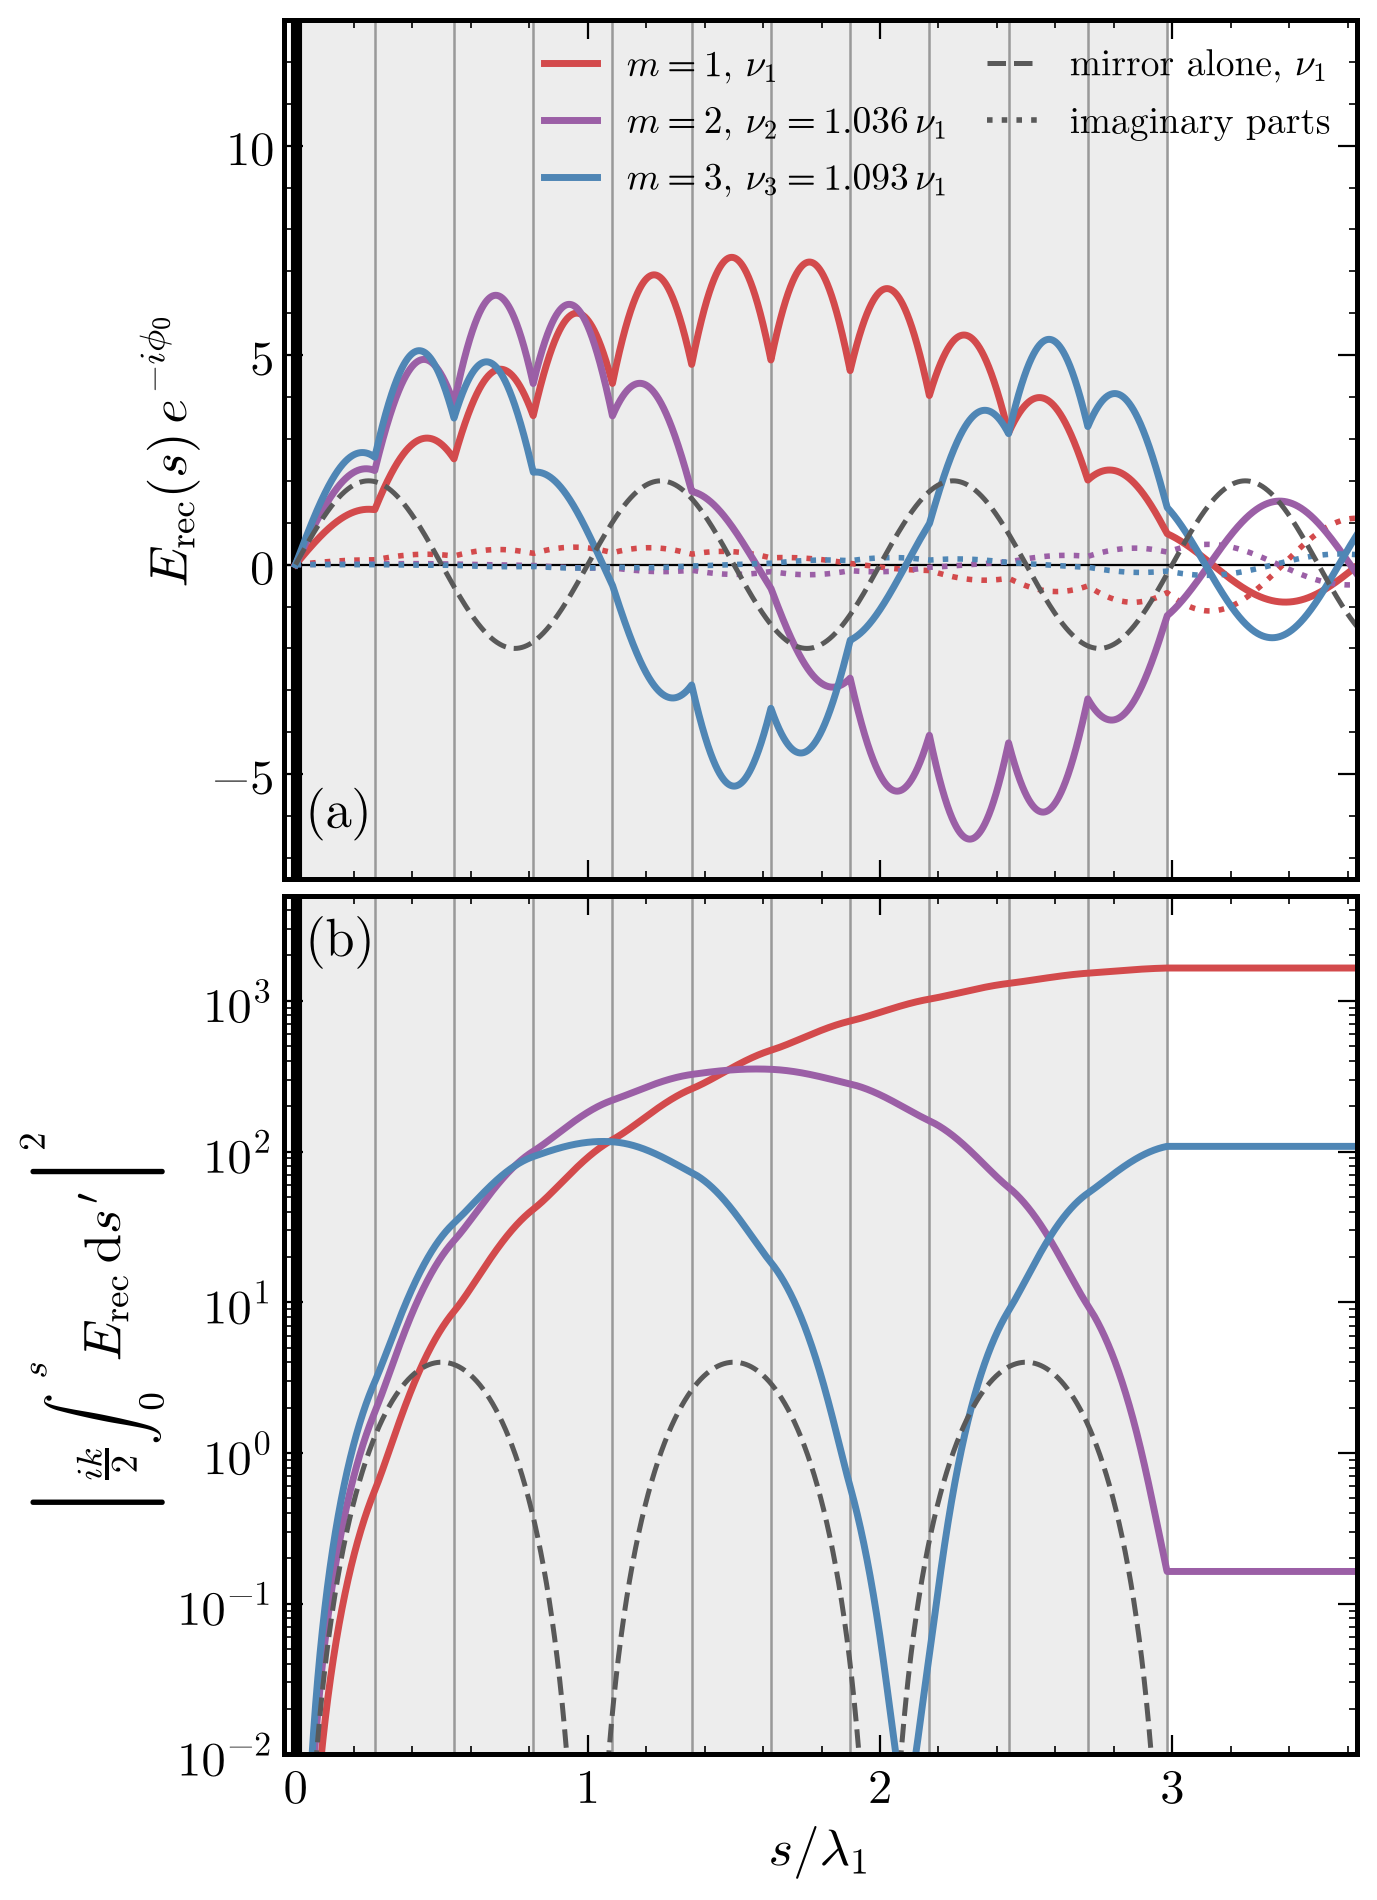
\includegraphics[width=\columnwidth]{fig_overlap_modes.png}
\caption{Receiving mode of the 1--2\,meV cartridge of Table~\ref{tab:design} ($N=11$, $d=a=238\,\mu$m, $r=0.03a$, $L=2.6$\,mm, impedance-sheet model). The distance from the mirror, $s$, is in units of the vacuum wavelength $\lambda_1=0.88$\,mm at the fundamental resonance $\nu_1=342$\,GHz ($m_a=1.41$\,meV). The thick line marks the mirror, thin lines the grids and the shaded band the stack; the incident wave has unit amplitude. (a)~Real (solid) and imaginary (dotted) parts of $E_{\rm rec}$, after removing a constant phase $\phi_0$, for the first three resonances of the stack, $m=1,2,3$, and real part for the mirror alone. The imaginary part describes the small flow of power into the copper. For $m=1$ it is at most about 12\% of the real part, and $|\int_0^LE_{\rm rec}\,\dd s|/\int_0^L|E_{\rm rec}|\,\dd s=0.99$, so the fundamental mode is a standing wave of nearly uniform phase. (b)~The overlap integral of Eq.~\eqref{eq:overlap} with its upper limit at $s$. Beyond $s=L$ there is no source and the curves give $|\beta|^2$.}
\label{fig:overlap}
\end{figure}


The axion-driven field obeys $E''+k^2E=-k^2E_0$ inside the magnetized stack and $E''+k^2E=0$ outside, where $-E_0$ is the vacuum particular solution of End Matter A. The Green's function of this problem is built from two source-free solutions: $E_{\rm rec}$, which satisfies all the conditions at the mirror and the grids, and the outgoing wave $e^{ik(s-L)}$. Their Wronskian, evaluated outside the stack, is $2ik$, and for $s>L$ one finds $E(s)=\beta E_0e^{ik(s-L)}$ with
\begin{equation}
\beta=\frac{ik}{2}\int_0^L E_{\rm rec}(s)\,\dd s .
\label{eq:overlap}
\end{equation}
The integral runs over the region where the axion source acts. Its meaning is simple. A thin slice $\dd s$ of the uniform axion source is a small antenna, which in empty space would radiate a wave of amplitude $(k\,\dd s/2)E_0$ toward the detector. In the presence of the grids and the mirror, reciprocity states that the amplitude and phase with which this wave reaches the detector are those of $E_{\rm rec}$ at the position of the slice. The boost is therefore the sum of the contributions of all slices, each weighted by the receiving mode. Two ingredients make it large: the receiving mode must be strong inside the stack, and it must have the same phase throughout, so that the contributions add rather than cancel. Consequently the loaded quality factor and coupling measured by reflectometry do not by themselves determine the axion sensitivity of a multilayer, which also requires the sign structure of the receiving mode~\cite{Garutti:2026asa}. As a check, for a mirror alone Eq.~\eqref{eq:overlap} gives $\beta=(1-\cos kL)e^{ikL}$, the $\varepsilon=1$ limit of Eq.~\eqref{eq:betaslab}, and for the cartridges of Table~\ref{tab:design} it reproduces the direct solution of End Matter A to numerical precision. Equation~\eqref{eq:overlap} is the one-dimensional form of the overlap formalism for dielectric haloscopes~\cite{Ioannisian:2017srr,Millar:2016cjp}, and of the reciprocity approach of Refs.~\cite{Egge:2022gfp,Egge:2023cos}.


In front of a bare mirror the receiving mode is the familiar standing wave, which changes sign every half wavelength (dashed curves in Fig.~\ref{fig:overlap}). Neighboring half-wavelength layers contribute with opposite signs and cancel in pairs. However thick the converting region, at most one uncompensated half-wavelength layer remains, and $|\beta|^2$ never exceeds 4.

The stack then behaves like a string fixed at both ends. The field vanishes at the mirror, and at a resonance it nearly vanishes at the front face as well, since the internal amplitude produced by a unit incident wave is largest, about $2/n_{\rm eff}$ with $n_{\rm eff}$ the effective refractive index of the lattice, when the face sits at a node of the internal standing wave. The resonances are therefore standing waves that fit an integer number $m$ of half internal wavelengths across the stack, $KL\simeq m\pi$, where $K$ is the wave number inside the lattice, and the mode $m$ has $m-1$ nodes. Figure~\ref{fig:overlap}(a) shows the first three of them. Only the fundamental mode, $m=1$, keeps the same sign throughout the stack, so every slice of the source adds in phase and the overlap in panel~(b) grows steadily up to the peak boost of Table~\ref{tab:design}. The antisymmetric mode $m=2$ has two lobes of opposite sign that cancel almost exactly, so the axion barely excites it, even though it appears clearly as an absorption dip in reflection. For $m=3$ two of the three lobes cancel each other, which leaves a power boost about fifteen times smaller than that of the fundamental. This cancellation between lobes is the origin of the factor $1-\cos\phi$ in Eq.~\eqref{eq:betaslab}, which vanishes for even $m$.


The coherent fundamental mode requires the stack to contain only half an internal wavelength. In vacuum this would limit the converting region to $\lambda/2$, the thickness of the first lobe of the mirror's standing wave. The stack in Fig.~\ref{fig:overlap} is instead three vacuum wavelengths thick, so the wavelength inside must be about six times longer than in vacuum, which requires a permittivity of a few percent. This is the ENZ condition seen from the receiver. 



\end{document}